\section{Schemes}
\label{sec:schemes}

In this section, we will present the schemes used to solve the previously quasi-discretized equations \ref{eq:INS_steady_2D_discretized_convection} and \ref{eq:INS_steady_2D_discretized_diffusion}.

Those schemes are the "tools" that will allow us to bind the currently considered cell values with its neighbor's cell values.
This means that at the end of this section, we will have a set of coefficients (based on the scheme adopted) that will be used to assemble the solving matrix of the system.

To further clarify, what we want to achieve is to compute the following functions ($nb$ indicates a generic neighbor cell, one or more cells away from the current cell $P$):

\begin{align}
    u_P & = f(u_{nb}, v_{nb}, p_{nb}) \\
    v_P & = f(u_{nb}, v_{nb}, p_{nb})
\end{align}

As we will see, the result of the schemes will be a set of coefficients that will be used to compute the values of $u_P$ and $v_P$ based on the values of the neighbor cells.
In particular, the final form of the system will be:

\begin{align}
    A_P^u u_P & = \sum_{nb} A_{nb}^u u_{nb} + b_P^u \\
    A_P^v v_P & = \sum_{nb} A_{nb}^v v_{nb} + b_P^v
    \label{eq:coefficients_form_system}
\end{align}

Notice how there is no direct correlation between the $u$ and $v$ equations, that are instead coupled through the pressure term $p$.

Using the indices' notation system $(i,j)$ becomes:

\begin{align}
    (A_P^u)_{i,j} u_{i,j} & = \sum_{nb} (A_{nb}^u)_{i,j} u_{i,j} + (p_{i,j} - p_{i+1,j}) \Delta y \\
    (A_P^v)_{i,j} v_{i,j} & = \sum_{nb} (A_{nb}^v)_{i,j} v_{i,j} + (p_{i,j} - p_{i,j+1}) \Delta x
\end{align}

Similar to the approach used in the previous section, we will treat separately the convection and diffusion terms.
In this way we will obtain two different sets of coefficients, one for the convection term and one for the diffusion term.
Those coefficients will be then reassembled together to reduce the equations to the final form presented above.

In particular, we will have that the coefficients $A_P^\phi$ and $A_{nb}^\phi$ will be the difference between the convection and diffusion coefficients, given that from Equation \ref{eq:FVM_momentum_x_direction}, we know:

\begin{equation}
    FVM_{\text{Convection}} - FVM_{\text{Diffusion}} = 0 \rightarrow (A^\phi) = (A^\phi)_{\text{Convection}} - (A^\phi)_{\text{Diffusion}}
\end{equation}

\textbf{Note:} In the following sections, we will refer to the use of \texttt{Mathematica}.
The complete notebook used to obtain the final form of the coefficients is left in the \ref{sec:appendix} section of this document.

\subsection{Convection schemes}
\label{subsec:convection_schemes}

In this section, we will present the schemes related to the convection terms of the discretized governing equations, which were derived in Section \ref{subsec:application_of_the_finite_volume_method}.



%
% USD scheme
%
\subsubsection{\acrfull{uds}}

The \acrfull{uds} is the simplest convection scheme, and it is a $1^{th}-order$ scheme.

The idea behind the \acrshort{uds} is to consider the velocity at the face of the $U_{CV}$ equal to the upwind value between the current cell center value and the neighbor cell center value.

This means that \acrshort{uds} scheme can be visualized as:

\begin{figure}[H]
    \centering
    \begin{tikzpicture}

        \draw[->] (-0.5,0) -- (5,0) node[right] {$x$};
        \draw[->] (0,-1) -- (0,3) node[above] {$u(x)$};

        % \draw [blue, thick] plot [smooth] coordinates {(-0.5,1) (2.5,2) (4.5,-0.5)};

        \draw (0,0) node[below left] {$u_{WW}$} -- (0,1.22);
        \draw (0.5,0) node[below, shift={(0,-10pt)}] {$u_{ww}$} -- (0.5,0);
        \draw (1,0) node[below] {$u_W$} -- (1,1.68);
        \draw (1.5,0) node[below, shift={(0,-10pt)}] {$u_w$} -- (1.5,0);
        \draw (2,0) node[below] {$u_P$} -- (2,1.98);
        \draw (2.5,0) node[below, shift={(0,-10pt)}] {$u_e$} -- (2.5,0);
        \draw (3,0) node[below] {$u_E$} -- (3,1.62);
        \draw (3.5,0) node[below, shift={(0,-10pt)}] {$u_{ee}$} -- (3.5,0);
        \draw (4,0) node[below] {$u_{EE}$} -- (4,0.3);


        \filldraw[red] (0,1.22) circle (1pt);
        \filldraw[red] (1,1.68) circle (1pt);
        \filldraw[red] (2,1.98) circle (1pt);
        \filldraw[red] (3,1.62) circle (1pt);
        \filldraw[red] (4,0.3) circle (1pt);

        \draw [red] (0.5,1.68) -- (1,1.68);
        \draw [red] (1.5,1.98) -- (2,1.98);
        \draw [red] (2,1.98) -- (2.5,1.98);
        \draw [red] (3,1.62) -- (3.5,1.62);

        % Legend
        % \draw [blue] (5.5,2) -- (6,2) node[right] {Actual $\hat{u(x)}$};
        \draw [red] (5.5,1.5) -- (6,1.5) node[right] {Computed $u(x)$ using \acrshort{uds}};

    \end{tikzpicture}
    \caption{Example of the \acrshort{uds} scheme applied to the $u$ velocity component.}
    \label{fig:uds_convection_scheme}
\end{figure}

We can obtain a formula for the \acrshort{uds} that will be used in the implementation of the code.
In particular, by defining the Volume Fluxes as: $F_e = \hat{u_e} \Delta y$ \& $F_w = \hat{u_w} \Delta y$, we can write that:

\begin{align}
    u_e & = \begin{cases}
                u_P & \text{if } F_e > 0 \\
                u_E & \text{if } F_e < 0
            \end{cases} \\
    u_w & = \begin{cases}
                u_W & \text{if } F_w > 0 \\
                u_P & \text{if } F_w < 0
            \end{cases}
\end{align}

The same apply for the $v$ velocity component, but in this case, we will have $F_n = \hat{v_n} \Delta x$, $F_s = \hat{v_s} \Delta x$.

In the end, our \acrfull{uds} scheme applied to the convection term will be:

\begin{gather*}
    \left(\hat{u_e}u_e - \hat{u_w}u_w\right) \Delta y + \left(\hat{v_n}u_n - \hat{v_s}u_s\right) \Delta x = \\
    \left(F_e u_e - F_w u_w\right) + \left(F_n u_n - F_s u_s\right) = \\
    u_P*max(F_e, 0) + u_E*min(F_e, 0) + u_W*max(F_w, 0) + u_P*min(F_w, 0) + \\
    u_P*max(F_n, 0) + u_N*min(F_n, 0) + u_S*max(F_s, 0) + u_P*min(F_s, 0)
\end{gather*}

Since we are interested in the $A_P^\phi$ and $A_{nb}^\phi$ coefficients as written in the form of Equation \ref{eq:coefficients_form_system}, with the help of \texttt{Mathematica}, we can regroup the terms based on the velocity components, perform some sign manipulations and obtain the coefficients for the convection term using the \acrshort{uds} scheme for both the $u$ and $v$ momentum equations.

\begin{equation}
    \text{Convection Coefficients \acrshort{uds}:} = { \textbf{See table \ref{tab:Ap_coefficients}} }
\end{equation}



%
% QUICK scheme
%
\subsubsection{\acrfull{quick}}

The \acrfull{quick} is a $3^{rd}-order$ scheme.

The idea behind the \acrshort{quick} scheme is to interpolate the velocity at the center of 3 cells to then compute the velocity at the face of the cell.
The choice of the cells to interpolate is based on the direction of the velocity at previous step ($\hat{u}$ or $\hat{v}$) similarly to the \acrshort{uds} scheme.
For example, if we are computing the $u_e$ velocity, we will pick as interpolations points the $u_P$, $u_E$ velocity and $u_{EE}$ or $u_{W}$ based on the direction of the velocity at the face.

The \acrshort{quick} scheme can be visualized as:

\begin{figure}[H]
    \centering
    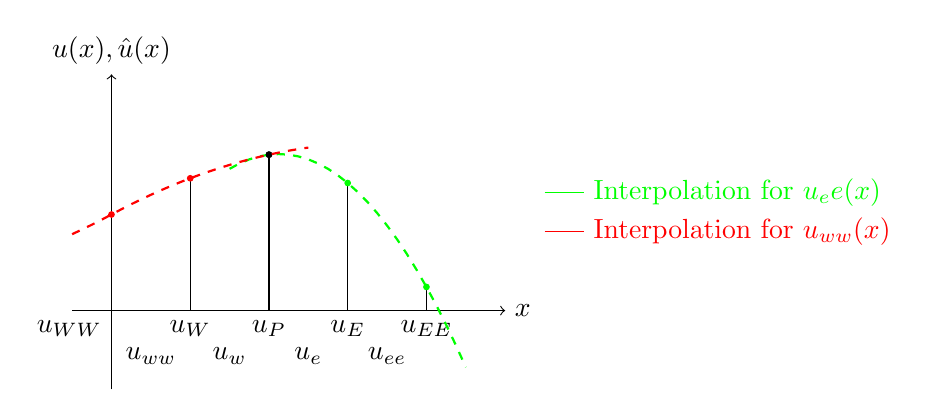
\begin{tikzpicture}

        \draw[->] (-0.5,0) -- (5,0) node[right] {$x$};
        \draw[->] (0,-1) -- (0,3) node[above] {$u(x), \hat{u}(x)$};

        % \draw [blue, thick] plot [smooth] coordinates {(-0.5,1) (2.5,2) (4.5,-0.5)};

        \draw (0,0) node[below left] {$u_{WW}$} -- (0,1.22);
        \draw (0.5,0) node[below, shift={(0,-10pt)}] {$u_{ww}$} -- (0.5,0);
        \draw (1,0) node[below] {$u_W$} -- (1,1.68);
        \draw (1.5,0) node[below, shift={(0,-10pt)}] {$u_w$} -- (1.5,0);
        \draw (2,0) node[below] {$u_P$} -- (2,1.98);
        \draw (2.5,0) node[below, shift={(0,-10pt)}] {$u_e$} -- (2.5,0);
        \draw (3,0) node[below] {$u_E$} -- (3,1.62);
        \draw (3.5,0) node[below, shift={(0,-10pt)}] {$u_{ee}$} -- (3.5,0);
        \draw (4,0) node[below] {$u_{EE}$} -- (4,0.3);

        % u_ee interpolation
        \filldraw[black] (2,1.98) circle (1pt);
        \filldraw[green] (3,1.62) circle (1pt);
        \filldraw[green] (4,0.3) circle (1pt);
        \draw [green, thick, dashed] plot[domain=1.5:4.5] (\x, {-0.48*\x^2 + 2.04*\x - 0.18});

        % w_ww interpolation
        \filldraw[red] (0,1.22) circle (1pt);
        \filldraw[red] (1,1.68) circle (1pt);
        \filldraw[black] (2,1.98) circle (1pt);
        \draw [red, thick, dashed] plot[domain=-0.5:2.5] (\x, {-0.08*\x^2 + 0.54*\x + 1.22});

        % Legend
        % \draw [blue] (5.5,2) -- (6,2) node[right] {Actual $\hat{u}(x)$};
        \draw [green] (5.5,1.5) -- (6,1.5) node[right] {Interpolation for $u_ee(x)$};
        \draw [red] (5.5,1) -- (6,1) node[right] {Interpolation for $u_{ww}(x)$};

    \end{tikzpicture}
    \caption{Example of the \acrshort{quick} scheme applied to the $u$ velocity component.}
    \label{fig:quick_convection_scheme}
\end{figure}

We can obtain a formula for the \acrshort{quick} that will be used in the implementation of the code.
In particular, we can recall the definition of the Lagrange interpolation polynomial of degree 2:

\begin{equation}
    P(x) = \sum_{i=0}^{2} y_i \prod_{j=0, j \neq i}^{2} \frac{x - x_j}{x_i - x_j}
    \label{eq:langrange_interpolation_polynomial}
\end{equation}

In our case, it's convenient to fix the reference system in correspondence of the center of the control volume considered.
If that is the case, then for example the evaluation of the velocity at the face $u_e$ will be:

\begin{equation}
    u_e = P(x) \bigg|_{x = \Delta x/2}
\end{equation}

As we said before, the choice of the interpolation points is based on the direction of the velocity at the face of the control volume.
In particular, if we are computing the $u_e$ velocity, the possible polynomials ($P_e(x)$) will be:

\begin{equation}
    P_e(x) = \begin{cases}
        P(u_W, u_P, u_E)    & \text{if } \hat{u_e} > 0 \\
        P(u_P, u_E, u_{EE}) & \text{if } \hat{u_e} < 0
    \end{cases}
\end{equation}

By using \texttt{Mathematica}, we can compute the polynomials for the $u$ velocity component in both cases.

The results of the symbolic analysis are:

\begin{align}
    u_e & = \begin{cases}
                -\frac{1}{8} u_W + \frac{3}{4} u_P + \frac{3}{8} u_E    & \text{if } \hat{u_e} > 0 \\
                +\frac{3}{8} u_P + \frac{3}{4} u_E - \frac{1}{8} u_{EE} & \text{if } \hat{u_e} < 0
            \end{cases}    \\
    u_w & = \begin{cases}
                -\frac{1}{8} u_{WW} +    \frac{3}{4} u_W + \frac{3}{8} u_P & \text{if } \hat{u_w} > 0 \\
                +\frac{3}{8} u_W + \frac{3}{4} u_P - \frac{1}{8} u_E       & \text{if } \hat{u_w} < 0
            \end{cases}
\end{align}

The same apply for the $v$ velocity component, but in this case, the variables that decide the interpolation points are the $\hat{v_n}$ and $\hat{v_s}$.

In the end, our \acrshort{quick} scheme applied to the convection term will be:

\begin{gather}
    \left(\hat{u_e}u_e - \hat{u_w}u_w\right) \Delta y + \left(\hat{v_n}u_n - \hat{v_s}u_s\right) \Delta x = \\
    \left(F_e u_e - F_w u_w\right) + \left(F_n u_n - F_s u_s\right) = \\
    \frac{1}{8} (
    (3 u_{E} + 6 u_{P} - u_{W}) max(0, F_e) + (- u_{EE} + 6 u_{E} + 3 u_{P}) min(0, F_e) + \\
    (- 3 u_{P} - 6 u_{W} + u_{WW}) max(0, F_w) + (u_{E} - 6 u_{P} - 3 u_{W}) min(0, F_w) + \\
    (3 u_{N} + 6 u_{P} - u_{S}) max(0, F_n) + (6 u_{N} - u_{NN} + 3 u_{P}) min(0, F_n) + \\
    (- 3 u_{P} - 6 u_{S} + u_{SS}) max(0, F_s) + (u_{N} - 6 u_{P} - 3 u_{S}) min(0, F_s)
    )
\end{gather}

Since we are interested in the $A_P^\phi$ and $A_{nb}^\phi$ coefficients as written in the form of Equation \ref{eq:coefficients_form_system}, with the help of \texttt{Mathematica}, we can regroup the terms based on the velocity components, perform some sign manipulations and obtain the coefficients for the convection term using the \acrshort{quick} scheme for both the $u$ and $v$ momentum equations.

\begin{equation*}
    \text{Convection Coefficients \acrshort{quick}:} = { \textbf{See table \ref{tab:Ap_coefficients}} }
\end{equation*}



%
% Hybrid scheme
%
\subsubsection{\acrfull{hybrid}}

The \acrfull{hybrid} combines the \acrshort{uds} and \acrshort{quick} schemes based on the Peclet number $P_e$.


\subsection{Diffusion Schemes}
\label{subsec:diffusion_schemes}

In this section, we will present the schemes related to the diffusion terms of the discretized governing equations, which were derived in Section \ref{subsec:application_of_the_finite_volume_method}.

The general idea here is to approximate the diffusion term using its Taylor expansion and then evaluate the derivative at the cell faces.
As a recall, the definition of the Taylor expansion of order $n$ is:

\begin{equation}
    f(x) = f(x_0) + f'(x_0)(x - x_0) + \frac{f''(x_0)}{2!}(x - x_0)^2 + \dots + \frac{f^n(x_0)}{n!}(x - x_0)^n + \mathbf{O}((x - x_0)^{n+1})
\end{equation}



%
% 2°-order scheme
%
\subsubsection{$2^{nd}$-order scheme}

The $2^{nd}$-order scheme approximate the diffusion term using the Taylor expansion up to the second order.

We can start by writing the polynomial that approximates by interpolation the values of the variable $u$ at the cell faces.
To do so, we can use the Lagrange interpolation polynomial, previously defined in Equation \ref{eq:langrange_interpolation_polynomial}.
Since we are now analyzing the $2^{nd}$-order scheme, we will use $n = 2+1 = 3$ points to interpolate.

As before, we can use \texttt{Mathematica} to obtain the polynomial that approximates function $u(x)$ as:

\begin{equation}
    u(x) \approx \frac{2 (\Delta x)^2 u_{P}+x^2 (u_{E}-2 u_{P}+u_{W})+\Delta x x (u_{E}-u_{W})}{2 (\Delta x)^2}
\end{equation}

We can now proceed by evaluating the second derivative of the polynomial as:

\begin{equation}
    \frac{\partial^2 u}{\partial x^2} \approx \frac{u_{E} - 2 u_{P} + u_{W}}{(\Delta x)^2}
\end{equation}

And finally, we can the approximated second derivative at the point of interest $x = 0$ as:

\begin{equation}
    \left. \frac{\partial^2 u}{\partial x^2} \right|_P \approx \frac{u_{E} - 2 u_{P} + u_{W}}{(\Delta x)^2}
\end{equation}

Given the definition of the diffusion term of $u$ along $x$ in Equation \ref{eq:INS_steady_2D_discretized_diffusion}, we can write the $2^{nd}$-order scheme as:

\begin{equation}
    \nu \frac{\partial^2 u}{\partial x^2} = \nu \frac{u_{E} - 2 u_{P} + u_{W}}{(\Delta x)^2}
\end{equation}

With a similar approach, we can obtain the $2^{nd}$-order scheme for the $y$ direction as:

\begin{equation}
    \nu \frac{\partial^2 u}{\partial y^2} = \nu \frac{u_{N} - 2 u_{P} + u_{S}}{(\Delta y)^2}
\end{equation}

The same procedure can be applied to the $v$ momentum equation, obtaining the following results:

\begin{gather}
    \nu \frac{\partial^2 u}{\partial x^2} + \nu \frac{\partial^2 u}{\partial y^2} = \\
    \frac{\Delta y \nu  (u_{E}-2 u_{P}+u_{W})}{\Delta x} + \\
    \frac{\Delta x \nu  (u_{N}-2 u_{P}+u_{S})}{\Delta y}
\end{gather}

Since we are interested in the $A_P^\phi$ and $A_{nb}^\phi$ coefficients as written in the form of Equation \ref{eq:coefficients_form_system}, with the help of \texttt{Mathematica}, we can regroup the terms based on the velocity components, perform some sign manipulations and obtain the coefficients for the diffusion term using the $2^{nd}$-order scheme for both the $u$ and $v$ momentum equations.

\begin{equation}
    \text{Diffusion Coefficients order} 2^{nd} = { \textbf{See table \ref{tab:Ap_coefficients}} }
\end{equation}



%
% 4°-order scheme
%
\subsubsection{$4^{th}$-order scheme}

The $4^{th}$-order scheme approximate the diffusion term using the Taylor expansion up to the fourth order.

Since the reasoning is similar to the $2^{nd}$-order scheme, we can directly write the approximated second derivative at the point of interest $x = 0$ as:

\begin{equation}
    \left. \frac{\partial^2 u}{\partial x^2} \right|_P \approx -\frac{u_{WW} - 16 u_{W} + 30 u_{P} - 16 u_{E} + u_{EE}}{12 (\Delta x)^2}
\end{equation}

Given the definition of the diffusion term of $u$ along $x$ in Equation \ref{eq:INS_steady_2D_discretized_diffusion}, we can write the $4^{th}$-order scheme as:

\begin{equation}
    \nu \frac{\partial^2 u}{\partial x^2} = \nu -\frac{u_{WW} - 16 u_{W} + 30 u_{P} - 16 u_{E} + u_{EE}}{12 (\Delta x)^2}
\end{equation}

With a similar approach, we can obtain the $4^{th}$-order scheme for the $y$ direction as:

\begin{equation}
    \nu \frac{\partial^2 u}{\partial y^2} = \nu -\frac{u_{WW} - 16 u_{W} + 30 u_{P} - 16 u_{E} + u_{EE}}{12 (\Delta y)^2}
\end{equation}

The same procedure can be applied to the $v$ momentum equation, obtaining the following results:

\begin{gather}
    \int_{V} \nu \frac{\partial^2 u}{\partial x^2} + \nu \frac{\partial^2 u}{\partial y^2} \space dV = \\
    -\frac{\nu}{12}  \left(\frac{u_{WW} - 16 u_{W} + 30 u_{P} - 16 u_{E} + u_{EE}}{(\Delta x)^2} + \frac{u_{WW} - 16 u_{W} + 30 u_{P} - 16 u_{E} + u_{EE}}{(\Delta y)^2} \right) \Delta x \Delta y
\end{gather}

Since we are interested in the $A_P^\phi$ and $A_{nb}^\phi$ coefficients as written in the form of Equation \ref{eq:coefficients_form_system}, with the help of \texttt{Mathematica}, we can regroup the terms based on the velocity components, perform some sign manipulations and obtain the coefficients for the diffusion term using the $4^{th}$-order scheme for both the $u$ and $v$ momentum equations.

\begin{equation}
    \text{Diffusion Coefficients order } 4^{th} = { \textbf{See table \ref{tab:Ap_coefficients}} }
\end{equation}

\subsection{Final coefficients}
\label{subsec:final_coefficients}

The final coefficients are obtained by reassembling the convection and diffusion coefficients, based on the FVM result:

\begin{equation}
    FVM_{\text{Convection}} - FVM_{\text{Diffusion}} = 0 \rightarrow (A^\phi) = (A^\phi)_{\text{Convection}} - (A^\phi)_{\text{Diffusion}}
\end{equation}


\eject
\newgeometry{margin=12mm}
\pdfpagewidth=275mm \pdfpageheight=150mm

\begin{center}
    \begin{table}[H]
        \centering
        \caption{Final $Ap$ coefficients for convection and diffusion using different schemes}
        \begin{tabular}{|l|l|l|l|l|l|}
            \hline
            \textbf{Ap}   & \textbf{Convection UDS} & \textbf{Convection CDS} & \textbf{Convection QUICK}                                                                     & \textbf{Diffusion 2° order}      & \textbf{Diffusion 4° order}          \\
            \hline
            $Ap\phi WWSS$ & $0$                     & $0$                     & $0$                                                                                           & $0$                              & $0$                                  \\
            $Ap\phi WWS$  & $0$                     & $0$                     & $0$                                                                                           & $0$                              & $0$                                  \\
            $Ap\phi WWP$  & $0$                     & $0$                     & $-\frac{1}{8} \max (0,Fw\phi )$                                                               & $0$                              & $-\frac{\Delta y \nu }{12 \Delta x}$ \\
            $Ap\phi WWN$  & $0$                     & $0$                     & $0$                                                                                           & $0$                              & $0$                                  \\
            $Ap\phi WWNN$ & $0$                     & $0$                     & $0$                                                                                           & $0$                              & $0$                                  \\
            $Ap\phi WSS$  & $0$                     & $0$                     & $0$                                                                                           & $0$                              & $0$                                  \\
            $Ap\phi WS$   & $0$                     & $0$                     & $0$                                                                                           & $0$                              & $0$                                  \\
            $Ap\phi WP$   & $\max (0,Fw\phi )$      & $\frac{Fw\phi}{2}$      & $\frac{1}{8} \max (0,Fe\phi )+\frac{3}{4} \max (0,Fw\phi )+\frac{3}{8} \min (0,Fw\phi )$      & $\frac{\Delta y \nu }{\Delta x}$ & $\frac{4 \Delta y \nu }{3 \Delta x}$ \\
            $Ap\phi WN$   & $0$                     & $0$                     & $0$                                                                                           & $0$                              & $0$                                  \\
            $Ap\phi WNN$  & $0$                     & $0$                     & $0$                                                                                           & $0$                              & $0$                                  \\
            $Ap\phi PSS$  & $0$                     & $0$                     & $-\frac{1}{8} \max (0,Fs\phi )$                                                               & $0$                              & $-\frac{\Delta x \nu }{12 \Delta y}$ \\
            $Ap\phi PS$   & $\max (0,Fs\phi )$      & $\frac{Fs\phi}{2}$      & $\frac{1}{8} \max (0,Fn\phi )+\frac{3}{4} \max (0,Fs\phi )+\frac{3}{8} \min (0,Fs\phi )$      & $\frac{\Delta x \nu }{\Delta y}$ & $\frac{4 \Delta x \nu }{3 \Delta y}$ \\
            \hline
            % $Ap\phi PP$   & $\max (0,Fe\phi )+\max (0,Fn\phi )-\min (0,Fs\phi )-\min (0,Fw\phi )$ & $\frac{Fe\phi}{2}+\frac{Fn\phi}{2}-\frac{Fs\phi}{2}-\frac{Fw\phi}{2}$ & $\frac{3}{4} \max (0,Fe\phi )+\frac{3}{8} \min (0,Fe\phi )+\frac{3}{4} \max (0,Fn\phi )+\frac{3}{8} \min (0,Fn\phi )-\frac{3}{8} \max (0,Fs\phi )-\frac{3}{4} \min (0,Fs\phi )-\frac{3}{8} \max (0,Fw\phi )-\frac{3}{4} \min (0,Fw\phi )$ & $-\Delta x \Delta y \nu  \left(-\frac{2}{\Delta x^2}-\frac{2}{\Delta y^2}\right)$ & $-\Delta x \Delta y \nu  \left(-\frac{5}{2 \Delta x^2}-\frac{5}{2 \Delta y^2}\right)$ \\
            $Ap\phi PP$   & $\sum_{nb} Ap\phi$      & $\sum_{nb} Ap\phi$      & $\sum_{nb} Ap\phi$                                                                            & $\sum_{nb} Ap\phi$               & $\sum_{nb} Ap\phi$                   \\
            \hline
            $Ap\phi PN$   & $-\min (0,Fn\phi )$     & $-\frac{Fn\phi}{2}$     & $\frac{1}{8} (-3) \max (0,Fn\phi )-\frac{3}{4} \min (0,Fn\phi )-\frac{1}{8} \min (0,Fs\phi )$ & $\frac{\Delta x \nu }{\Delta y}$ & $\frac{4 \Delta x \nu }{3 \Delta y}$ \\
            $Ap\phi PNN$  & $0$                     & $0$                     & $\frac{1}{8} \min (0,Fn\phi )$                                                                & $0$                              & $-\frac{\Delta x \nu }{12 \Delta y}$ \\
            $Ap\phi ESS$  & $0$                     & $0$                     & $0$                                                                                           & $0$                              & $0$                                  \\
            $Ap\phi ES$   & $0$                     & $0$                     & $0$                                                                                           & $0$                              & $0$                                  \\
            $Ap\phi EP$   & $-\min (0,Fe\phi )$     & $-\frac{Fe\phi}{2}$     & $\frac{1}{8} (-3) \max (0,Fe\phi )-\frac{3}{4} \min (0,Fe\phi )-\frac{1}{8} \min (0,Fw\phi )$ & $\frac{\Delta y \nu }{\Delta x}$ & $\frac{4 \Delta y \nu }{3 \Delta x}$ \\
            $Ap\phi EN$   & $0$                     & $0$                     & $0$                                                                                           & $0$                              & $0$                                  \\
            $Ap\phi ENN$  & $0$                     & $0$                     & $0$                                                                                           & $0$                              & $0$                                  \\
            $Ap\phi EESS$ & $0$                     & $0$                     & $0$                                                                                           & $0$                              & $0$                                  \\
            $Ap\phi EES$  & $0$                     & $0$                     & $0$                                                                                           & $0$                              & $0$                                  \\
            $Ap\phi EEP$  & $0$                     & $0$                     & $\frac{1}{8} \min (0,Fe\phi )$                                                                & $0$                              & $-\frac{\Delta y \nu }{12 \Delta x}$ \\
            $Ap\phi EEN$  & $0$                     & $0$                     & $0$                                                                                           & $0$                              & $0$                                  \\
            $Ap\phi EENN$ & $0$                     & $0$                     & $0$                                                                                           & $0$                              & $0$                                  \\
            \hline
        \end{tabular}
        \label{tab:Ap_coefficients}
    \end{table}
\end{center}

\eject
\restoregeometry
\pdfpagewidth=210mm
\pdfpageheight=297mm
